\chapter{Proposta de solución}


Los archivos de registro de actividad que sobre los que se obtendrá la información del sistema se dividen en varios archivos, cada uno con un objetivo concreto. En concreto se monitorizarán tres ficheros, los cuales poseen un ciclo de vida que consiste en pasar por un fichero plano, para una vez alcanzado un tamaño determino comprimirse y guardarse como histórico. Si el histórico tiene una antigüedad superior a los días establecidos como máximo se enviarán a un servidor que funcionará como almacenamiento. Estos tres ficheros tienen los siguientes acometidos:

\begin{itemize}
\item Registro de interacciones (peticiones y respuestas) con otros sistemas externos e internos.
\item Registro de las transformaciones y cálculos que reciben los datos en los distintos servicios de los que se compone la aplicación.
\item Registro de la aplicación de entrada que utilizarán los usuarios finales con registro de las operaciones solicitadas y pantallas accedidas.
\end{itemize}

En los logs de actividad se registrarán el momento en que se registran, la clase en la que se originó el comportamiento y el texto con la información que se está registrando en ese momento.


En este capítulo se va a describir la plataforma implementada para la emisión de alertas. La arquitectura diseñada para la plataforma es la siguiente:

\begin{figure}[H]
\centerline{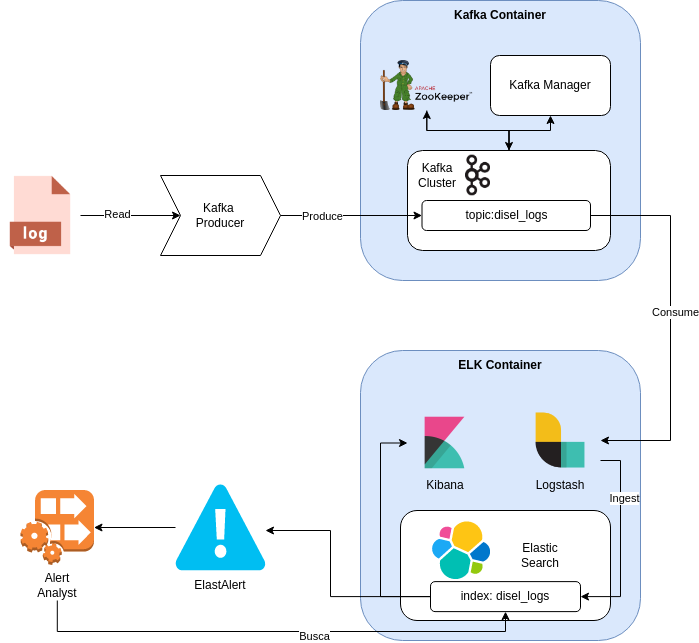
\includegraphics[width=15cm]{figuras/arquitectura.png}}
\caption{Arquitectura de la Plataforma de Gestión de Alertas}
\label{enlace1}
\end{figure}

La arquitectura estará desplegado en varios contenedores Docker. Se pueden distinguir las siguientes partes:

\begin{itemize}
\item \textbf{Producer}: como se ha comentado en el capítulo de introducción no es posible utilizar los logs de la aplicación real en el entorno de producción ya que se estaría incumpliendo la ley de protección de datos. Para ello se utilizarán logs ya registrados de los que se tiene certeza que se produjo una incidencia pero procedente de un entorno de desarrollo con datos falsos. Para reproducir el comportamiento de la aplicación se implementará un script python que se encargue de leer cada línea de log y trasladarla a kafka, de esta forma replicará el comportamiento de escribir regitros a lo largo del tiempo.

\item \textbf{Kafka server}: se utilizará kafka con el fin de trasladar los datos producidos en el productos al ELK Stack. La plataforma Apache Kafka es un sistema de transmisión de datos distribuido con capacidad de escalado y tolerante a fallos. Gracias a su alto rendimiento permitirá transmitir datos en tiempo real utilizando el patrón de mensajería publish/subscribe. 

\item \textbf{ELK Stack}: conjunto de aplicaciones (Elastic Search, Logstash y Kivana). Permite recoger datos de cualquier tpo de fuente y cualquier formato para realizar búsquedas, análisis y visualización de los datos en tiempo real. En la arquitectura planteada se para la aplicación real se obtendrán los datos a partir de ficheros de logs mediante Logstash y se almacenarán en el motor de búsquedas y análisis de Elasticsearch. Además, se permite la visualización, monitorización y explotación de datos en tiempo real mediante kibana.

\item \textbf{Elastalert}: herramienta open source que se integra con ELK y permite detectar anomalías e inconsistencias en los datos de Elasticsearch y lanzar alertas. El conjunto de herramientas de \textbf{ELK (Elastic Stack)} más ElastAlert permite crear un sistema de monitorización para la extracción, almacenamiento y explotación de los datos de los procesos o sistemas a monitorizar.

\end{itemize}
